\documentclass[a4paper,11pt]{report}
\usepackage[]{amsmath}
\usepackage[]{physics} % \bra, \ket etc
\usepackage{graphicx} %Pour les figures je crois
\usepackage{hyperref}
\usepackage[
    backend=biber, 
    natbib=true,
    style=numeric-comp,
    sorting=none, %Pour faire apparaitre les refs dans l'ordre
    hyperref=true
]{biblatex} %Imports biblatex package
\addbibresource{Bib_ch4.bib} %Import the bibliography file

\usepackage{amssymb} %quelques symboles dont gtrsim /lesssim
\usepackage{subcaption} % package pour faire des subfigures
\usepackage{multirow} % package pour multirow/multicolumn
\usepackage{booktabs} % package pour top/mid/bottom rule
\usepackage{tcolorbox} % toujours plus de boites
\usepackage{xcolor} % Pour avoir des couleurs dans les équations

\title{}
\begin{document}
\chapter{NV-NV CR under transverse or low fields: application to magnetometry}

(mentionner l'article ici !).... The main motivation for this study was the potential to use NV-NV CR as a low field magnetometry protocol. Indeed, while NV-NV CR lines can be used to perform magnetometry with non zero fields [les russes], there are several advantages to use NV-NV CR as close to the zero magnetic field region, in particular the non dependence of the magnetic field orientation with respect to the crystal lattice. The behavior of 

\section{NV spin Hamiltonian under low and transverse fields}

Before looking at the NV-NV CR in the low or transverse field regime, we first need to consider how the general NV physics is modified under those regimes, and in particular we need to look at the modifications of the spin Hamiltonian and the change in the eigenstates.

\subsection{NV spin Hamiltonian in zero external magnetic field}
\begin{figure}[h]
\centering
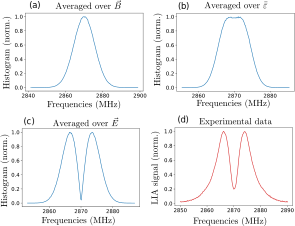
\includegraphics[width=\textwidth]{Figures/ESR_simus}
\caption{Simulations of inhomogeneous zero field ODMR when sampling various parameters. a) Simulation when sampling each components of the magnetic field over a Gaussian of deviation $\sigma=2\ \rm G$. b) Simulation when sampling each components of the strain tensor $\bar{\bar{\varepsilon}}$ over a Gaussian of deviation $\sigma=2\cdot 10^{-4}$. c) Simulation when sampling each components of the electric field over a Gaussian of deviation $\sigma=2\cdot 10^{5}\ \rm{V/cm}$. d) Experimental ODMR spectrum in zero external field taken on sample ADM-150-2}
\label{simus ESR}
\end{figure}

In the absence of external magnetic field, we have to take into account other elements which would otherwise be of second order in the spin Hamiltonian. These elements are: the random local magnetic fields caused by paramagnetic impurities, the local electric field caused by charged impurities, and the crystal strain \citep{doherty2012theory, udvarhelyi2018spin, mittiga2018imaging}. The hyperfine splitting due to nearby nuclei will be considered separately, although to a large extent it behaves like a local magnetic field.

Due to the large zero field splitting $D=2870 MHz$ between the $\ket{0}$ and $\ket{\pm 1}$ states, we will consider the $\ket{0}$ to always be an eigenstate of the spin Hamiltonian under zero external field (which is equivalent to say that we neglect the terms in $\ket{0}\bra{\pm 1}$ in the spin Hamiltonian). The problem is then reduced to the $\{ \ket{-1}, \ket{+1} \}$ subsystem.

The NV$^-$spin Hamiltonian in the $\{ \ket{-1}, \ket{+1} \}$ basis can be written as \citep{udvarhelyi2018spin}:
\begin{equation}
\mathcal{H}=\begin{pmatrix}
D-\gamma_e B_\parallel + f_\parallel(\mathbf{E}) + g_\parallel(\bar{\bar{\varepsilon}}) & f_\perp(\mathbf{E}) + g_\perp(\bar{\bar{\varepsilon}})\\
f^*_\perp(\mathbf{E}) + g^*_\perp(\bar{\bar{\varepsilon}})&D+\gamma_e B_\parallel + f_\parallel(\mathbf{E}) + g_\parallel(\bar{\bar{\varepsilon}})
\end{pmatrix},
\label{Hamiltonien pm1}
\end{equation}
where $B_\parallel$ is the component of the magnetic field along the NV axis, and $f_\parallel, f_\perp, g_\perp$, and $g_\parallel$ are functions of the electric field $\mathbf{E}$ and the strain tensor $\bar{\bar{\varepsilon}}$, whose expressions are:

\begin{align}
f_\parallel(\mathbf{E})&=d_\parallel E_z, \\
f_\perp(\mathbf{E})&=d_\perp ( E_x + i E_y), \\
g_\parallel(\bar{\bar{\varepsilon}})&= h_{41}(\varepsilon_{xx}+\varepsilon_{yy})+h_{43} \varepsilon_{zz}, \\
g_\perp(\bar{\bar{\varepsilon}}) &= \frac{1}{2} \left[ h_{16}(\varepsilon_{zx}+i \varepsilon_{zy}) + h_{15}\left(\frac{\varepsilon_{yy}-\varepsilon_{xx}}{2}+i\varepsilon_{xy}\right) \right],
\end{align}
where $d_\parallel=0.35 \ \rm{Hz\, cm/V}$ and $d_\perp=17\ \rm{Hz\, cm/V}$ have been measured experimentally \citep{van1990electric}, and $h_{43}=2300\ \rm{MHz}$, $h_{41}=-6420\ \rm{MHz}$, $h_{15}=5700\ \rm{MHz}$ and $h_{16}=19660\ \rm{MHz}$ were computed through DFT \citep{udvarhelyi2018spin} and show reasonable agreement with experiments \citep{barson2017nanomechanical}.

Importantly, as pointed in \citep{mittiga2018imaging} we notice that both the electric field and the strain have a \textit{shifting} component ($f_\parallel$ and $g_\parallel$) which shifts equally both eigenstates of the Hamiltonian, and a \textit{splitting} component ($f_\perp$ and $g_\perp$) which splits in energy the two eigenstates. 

The main difference between the electric field and the strain is in the numerical prefactors of these components: for the electric field, the splitting parameter $d_\perp$ is $\sim 50$ times higher than the shifting parameter $d_\parallel$, which will result on average to a strong energy split without much shifting. For the strain however, the splitting parameters $h_{15}$ and $h_{16}$ are only $\sim 3$ times higher than the shifting parameters $h_{43}$ and $h_{41}$. The shift in energy will therefore tend to blur the energy split when averaging over a large number of spins.

Fig. \ref{simus ESR} shows a simulation of how each parameters of the spin Hamiltonian - local magnetic field, local electric field and strain - affects the zero external field ODMR profile. To do these simulations, I sampled each parameters separately $10^6$ times and plotted the histogram of the two eigenvalues of the Hamiltonian written in eq. \ref{Hamiltonien pm1}. Fig. \ref{simus ESR}-d) shows an experimental zero field ODMR spectrum, typical of what we observe with dense NV ensembles. 

Experimentally, almost all our samples show the characteristic two bumps in zero external field ODMR. Given the simulation results, the only parameter that can give rise to this shape is the electric field. We will therefore consider that the NV Hamiltonian of our samples is dominated by the local electric field, and more specifically by the transverse electric field $E_\perp\equiv E_x + i E_y$ given the ratio between $d_\perp$ and $d_\parallel$.

We will then adopt the following simplified Hamiltonian for the zero external field regime:
\begin{equation}
\mathcal{H}=\begin{pmatrix}
D&0&d_\perp E_\perp^* \\
0&0&0 \\
d_\perp E_\perp &0&D
\end{pmatrix},
\end{equation}
whose eigenvectors are $\ket{0}$ and$\ket{\pm}$ of eigenvalues 0 and $D\pm d_\perp \abs{E_\perp}$, where $\ket{\pm}$ are defined as:
\begin{equation}
\ket{\pm}=\frac{\ket{+1}\pm e^{-i\phi_E}\ket{-1}}{\sqrt{2}},
\end{equation}
where $\tan(\phi_E)=E_y/E_x$.

\subsection{NV spin Hamiltonian under purely transverse magnetic field}
\label{sec B transverse}
%\begin{figure}[h]
%\centering
%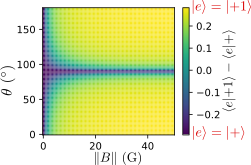
\includegraphics[width=0.7\textwidth]{Figures/map_etats_propres}
%\caption{Closeness of the Hamiltonian most excited state $\ket{3}$ with either $\ket{+1}$ or $\ket{+}$ as a function of the external magnetic field amplitude and angle $\theta$ with respect to the NV axis.}
%\label{map champ transverse}
%\end{figure}

We will consider here the case of purely transverse magnetic field with respect to the NV axis, i.e. $\mathbf{B}=B_x \hat{e}_x + B_y \hat e_y$, and more specifically the regime where $d_\perp E_\perp < \frac{(\gamma_e B_\perp)^2}{D} << D$. In practice, this generally means $20\ \rm G \lesssim B_\perp \lesssim 200\ \rm G$.

In this regime, the NV Hamiltonian eigenstates are similar to the case dominated by the transverse electric field and can be written $\approx \ket{0}, \ket{\pm}$\citep{qiu2021nuclear, qiu2022nanoscale}, of eigenvalues $\approx -\frac{(\gamma_e B_\perp)^2}{D},D$ and $D+\frac{(\gamma_e B_\perp)^2}{D}$,  where:
\begin{equation}
\ket{\pm}=\frac{\ket{+1}\pm e^{-2i\phi_B}\ket{-1}}{\sqrt{2}},
\end{equation}
and $\tan(\phi_B)=B_y/B_x$.

For the case where $d_\perp E_\perp \sim \frac{(\gamma_e B_\perp)^2}{D}$ and $\phi_E \neq 2\phi_B$, the eigenstates of the Hamiltonian are still $\ket{0},\ket{\pm}$ with a relative angle $\phi$ in between $\phi_E$ and $2\phi_B$.

In conclusion, whenever the spin Hamiltonian is dominated by a transverse field, either electric or magnetic, we can consider that the eigenstates of the spin Hamiltonian or $\ket{0}, \ket{-}$ and $\ket{+}$, whereas when the Hamiltonian is dominated by the longitudinal magnetic field, its eigenstates are $\ket{0}, \ket{-1}$ and $\ket{+1}$.

\subsection{Hyperfine coupling and inhomogeneous broadening}
\label{sec modif T2*}
\begin{figure}[h]
\centering
\includegraphics[width=\textwidth]{Figures/Comparaison_ESR_T2*}
\caption{tata. Changer les T1 avec T1ph=5ms}
\label{ESR for T2*}
\end{figure}

We will now look at the modification in the ODMR linewidths caused by the different magnetic field regimes. These change are relevant to our study of NV-NV CR due to the relation between the dipole-induced relaxation rate and $T_2^*$ detailed in sec. [REF].

A consequence of the change in the Hamiltonian eigenstates from the $\{ \ket{0}, \ket{\pm 1} \}$ to the $\{ \ket{0}, \ket{\pm} \}$ basis is that the Hamiltonian eigenvalues are sensitive to different part of the environment. In the $\{ \ket{0}, \ket{\pm 1} \}$, the eigen energies are linearly sensitive to (longitudinal) magnetic field, and only sensitive to electric fields at the second order, and vice versa for the $\{ \ket{0}, \ket{\pm} \}$ basis.

These different sensitivities affect both the inhomogeneous broadening, due to the local electric and magnetic noise, and the hyper-fine coupling to the various surrounding nuclei. These effects can drastically modify the ODMR lineshape in zero external magnetic field \citep{jamonneau2016competition} or purely transverse magnetic field \citep{qiu2021nuclear,qiu2022nanoscale}.

We will only consider here the hyper-fine splitting caused by the $^14$N nuclei of the nitrogen atom forming the NV center. $^14$N represents 99.6 \% of natural abundance nitrogen atoms, and it has an $I=1$ nuclear spin. The full $3\times 3$ Hamiltonian of the NV center in these conditions can be written:
\begin{equation}
\mathcal{H}=\mathcal{H}_e + \mathcal{H}_n + \mathbf{S} \bar{\bar{A}} \mathbf{I},
\end{equation}

where $\mathbf{S}$ is the electronic spin operator, $\mathbf{I}$ the nuclear spin operator, $\mathcal{H}_e$ the previously described electronic spin Hamiltonian, $\mathcal{H}_n$ the nuclear spin Hamiltonian and $\bar{\bar{A}}$ the hyper fine tensor. $\mathcal{H}_n$ and $\bar{\bar{A}}$ can be written:

\begin{align}
\bar{\bar{A}} &= \begin{pmatrix}
A_{xx} & 0 & 0 \\
0 & A_{yy} & 0 \\
0 & 0 & A_{zz}
\end{pmatrix} \\
\mathcal{H}_n &= \gamma_N \mathbf{I} \cdot \mathbf{B} + Q I_z^2,
\end{align}

where $\gamma_N=0.308\ \rm kHz/G$, $Q=-4.945\ \rm MHz$, $A_{zz}=-2.162\ \rm MHz$ and $A_{xx}=A_{yy}=-2.62\ \rm MHz$ \citep{smeltzer2009robust}.

Fig. \ref{ESR for T2*} shows ODMR spectra for two samples, CVD-pink and Sumi-2, in three magnetic configuration: for a strong longitudinal magnetic field, where the NV eigenbasis is $\{ \ket{0}, \ket{\pm 1} \}$, and for a strong transverse magnetic field or no magnetic field, where the NV eigenbasis is $\{ \ket{0}, \ket{\pm} \}$. A table with the full width at half maximum of each ODMR line is shown in Fig. \ref{ESR for T2*}-d)

While both samples are relatively equivalent in term of NV concentration ([NV]=$3 \sim 5$ ppm), sample Sumi-2, being a Type 1B HPHT sample, contains significantly more impurities besides NV centers, most likely P1 centers. These impurities cause both magnetic (because of paramagnetic impurities) and electric (because of charged impurities) field noise.

Fig. \ref{ESR for T2*}-a) allows us to evaluate the magnetic field noise in both samples, since the $\ket{\pm 1}$ states are not sensitive to weak electric fields. We indeed find that the Sumi-2 sample has much more magnetic noise, to the point where the hyper-fine structure is no longer resolved. The total width of the line however is mostly dominated by the hyper-fine splitting, which result in a similar total linewidth in both cases

We should note that the current practice in magnetometry is to consider only of the three hyper-fine lines when they are resolved. This is because magnetometry protocol usually relies on a microwave field with a very well defined frequency, which can effectively select only one of the lines. In our case however, we have to consider the spectral overlap between NV centers and fluctuators, which have an additional broadening of $2\gamma_f \approx 6\ \rm MHz$ [REF] that completely obscures the hyper-fine structure. We therefore have to consider the full linewidth, even when the hyper-fine structure is resolved.

Fig. \ref{ESR for T2*}-b) allows us to evaluate the electric field noise in both samples, since the $\ket{\pm}$ states are not sensitive to weak magnetic fields. Similarly, the hyper-fine structure is hidden in this configuration since all three hyper-fine levels are nearly-degenerate, provided that $\frac{(\gamma_e B_\perp)^2}{D} > A_{xx},A_{zz},Q$ which is typically the case for $B_\perp > 40\ \rm G$. We can note that the electric field noise is significantly stronger in the HPHT sample, which leads to an ODMR linewidth more than twice as big.

Finally, \ref{ESR for T2*}-c) shows the linewidth of both samples for zero external magnetic field. For sample Sumi-2, the profile and linewidth is similar to the case of the purely transverse magnetic field, which is consistent with the fact that the electric field noise is stronger than the residual magnetic fields (earth magnetic field and hyper-fine interaction). For sample CVD-pink however, the electric field noise is smaller than the hyper-fine interaction, meaning that only the $\ket{m_I=0}$ states (the ones closest to the central dip) will be dominated by the electronic noise, and be in the electronic states $\ket{m_e=\pm}$. The $\ket{m_I=\pm 1}$ states are dominated by the hyper-fine field and are in the electronic $\ket{m_e=\pm 1}$ basis.

Overall, we are mostly interested in the linewidth of the ODMR lines for various magnetic field conditions. While these linewidth are quite significantly changed for sample CVD-pink, the change is less pronounced on sample Sumi-2. Most HPHT samples we used are from type 1B diamond, and behave similarly to sample Sumi-2. Since almost all measurements in this chapter will be conducted on HPHT samples, we will consider the modification of $T_2^*$ as a minor effect.

\section{NV-NV CR in the low magnetic field regime}
In this part, we will study the cross-relaxation between NV centers whose spin Hamiltonian is dominated by a transverse field, either magnetic or electric. This is an important regime because it corresponds to the low magnetic field region where the electric field dominates, which is the region for which we want to implement our magnetometry protocol. We will also study here the double flip CR processes which we had neglected in the last chapter.

\subsection{NV-NV CR under low magnetic field}
\begin{figure}[h]
\centering
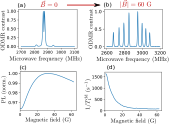
\includegraphics[width=0.9\textwidth]{Figures/scan_1x1x1x1}
\caption{tata. Changer les T1 avec T1ph=5ms}
\label{scan 1x1x1x1}
\end{figure}
We will start by showing that NV-NV CR behaves differently in the low magnetic field regime compared to the longitudinal field dominated regime which we studied in the last chapter.

The main issue with studying NV-NV CR in low to zero magnetic field is that there are many competing effects happening simultaneously, with few buttons to adjust to isolate each effects.

Fig. \ref{scan 1x1x1x1}-c) and d) for example shows the evolution of the NV PL and stretched lifetime $T_1^{\rm dd}$, defined in the last chapter [REF], as the magnetic field is scanned from 0 to 60 G. The ODMR at the initial and final magnetic fields are shown in Fig. \ref{scan 1x1x1x1}-a) and b).

While it is clear that the spin lifetime, as well as the PL, increases when the magnetic field, there is no clear indication that this is because of the specificity of the low field region. Indeed, the most likely explanation in this case is that the four classes of NV centers get split apart as the magnetic field increases, which reduces the density of resonant fluctuators for each NV centers.

\begin{figure}[h]
\centering
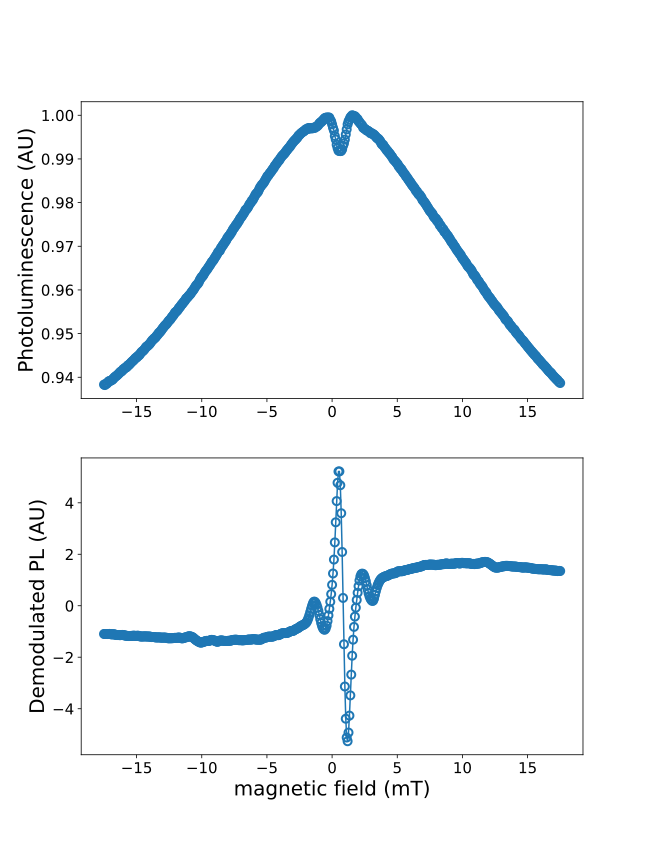
\includegraphics[width=0.9\textwidth]{Figures/scan_100}
\caption{Same measurements as Fig. \ref{scan 1x1x1x1}, still on sample ADM-150-1, but with $\mathbf{B}$ along the [100] axis. Changer les T1 avec T1ph=5ms}
\label{scan 100}
\end{figure}

Fig. \ref{scan 100} presents a way to circumvent this issue: by applying the magnetic field along the [100] crystalline axis, we can make sure that the four classes of NV centers always stay resonant regardless of the magnetic field amplitude.

We can notice that there still is a decrease of both the PL and $T_1^{\rm dd}$ in low field, although considerably smaller than the previous case: in Fig. \ref{scan 1x1x1x1}, $T_1^{\rm dd}$ was reduced by a factor of [REF] in zero field, whereas in Fig. \ref{scan 100}, it was only reduced by a factor of [REF]. The main reason for the PL and $T_1$ drop was indeed the co-resonance between the four classes.

Nevertheless, the fact that there is a drop in zero field when $\mathbf{B} \parallel [100]$ cannot be explained by using only the inter-class resonances. There are some additional depolarization mechanisms which are proper to the zero field region. We should also note that, while the zero-field PL contrast is bigger in Fig. \ref{scan 1x1x1x1}-c) than in Fig. \ref{scan 100}-c), the slope, which is the limiting factor for sensing ability, is actually very similar in both cases with a value $\sim [REF]\ \rm G^{-1}$.

\subsection{Potential causes for low field depolarization}

We will discuss here three possible reasons for the zero field depolarization observed in Fig. \ref{scan 100}. Once presented, we will try to hierarchized the contribution of each of these effects.

\subsubsection{Eigenstates modification}
The first explanation is the modification of the dipole-dipole interaction caused by the change of the NV Hamiltonian eigenbasis from $\{ \ket{0}, \ket{\pm 1} \}$ when $\mathbf{B} \neq 0$ to $\{ \ket{0}, \ket{\pm} \}$ when $\mathbf{B} = 0$.

This modification arise from the new form of the dipole-dipole Hamiltonian in the $\{ \ket{0}, \ket{+}, \ket{-} \} \times \{ \ket{0}, \ket{+}, \ket{-} \}$ basis. We justify this change of basis, which only consider the single NV Hamiltonian instead of the full Hamiltonian of the two coupled NV centers, by the fact that we are in the weak coupling regime, where $\expval{\mathcal{H}_{dd}} \approx 50\ \rm kHz \ll \frac{1}{2\pi T_2^*} \approx 5\ \rm MHz$.

To compute the decay rate in these case, similarly to what we did in sec. REF, we now need to consider the $\mel{0,\pm}{\mathcal{H}_{dd}}{\pm ,0}$ matrix elements instead of the $\mel{0,\pm 1}{\mathcal{H}_{dd}}{\pm 1,0}$ ones.

The averaging of these matrix elements, which is needed to compute the expected decay rates, is detailed in appendix [REF]. The computation in this case is complicated by the fact that the transverse field (either $\mathbf{E}$ or $\mathbf{B}$) responsible for the splitting of the $\ket{\pm}$ levels breaks the Hamiltonian symmetry in the $(xy)$ plane. This means that the dipole-dipole coupling between two spins will depend on their relative $x$ and $y$ axis, defined by the local transverse field, on top of the relative $z$ axis defined by the NV axis. 

We therefore need to make an assumption on the distribution of the transverse field in the sample. In zero external magnetic field where the dominant transverse field comes from randomly spaced charged impurities, we can expect the $x$ and $y$ axes to be randomly sampled in their respective $(xy)$ plane. However, since the NV-fluctuator CR is dominated by the closest neighbor of each spin (due to the $1/r^6$ scaling in eq. [REF]), there could still be local correlations in the transverse field felt by the NV and the fluctuator.

We then computed the decay rates for the two extreme cases: first, we consider that the $x$ and $y$ axis of each spin is randomly sampled, which correspond to a correlation length of the transverse field $l_c=0$, and secondly we considered the case where the $x$ and $y$ axes of every spin are the same, which correspond to $l_c=\infty$.

We found for $\mathbf{B}=0$ that the expected decay rate was $\Gamma_1=51.4 \Gamma_0^{th}$ if $l_c=0$ and $\Gamma_1=55.0 \Gamma_0^{th}$ if $l_c=\infty$. $\Gamma_0^{th}$ has the same definition as in table [REF], it is the expected CR rate for an isolated class in the $\{ \ket{0}, \ket{\pm 1} \}$ basis.

In both cases, this is a moderate ($\sim 20 \%$) increase compared to $\Gamma_1=42.8 \Gamma_0^{th}$ which we previously found for $\mathbf{B} \parallel [100]$, where all four classes are degenerate but the Hamiltonian eignebasis is $\{ \ket{0}, \ket{\pm 1} \}$. The change in the Hamiltonian eigenbasis for low field is therefore a possible candidate to explain the low field depolarization in Fig. \ref{scan 100}

\subsubsection{Double flips}

\begin{table}[htbp]
\centering
\caption{Simulated depolarization rate for flip-flops and double flips in zero magnetic field}
 \label{table double flips}
\begin{tabular}{c|cc}
%\toprule
{} & $l_c=0$ & $l_c=\infty$ \\
\midrule
$\bar{R}^2=1$ & $126.8 \Gamma_0^{\rm th}$ & $126.8 \Gamma_0^{\rm th}$ \\
$\bar{R}^2=0.5$ & $NA \Gamma_0^{\rm th}$ & $NA \Gamma_0^{\rm th}$ \\
$\bar{R}^2=0$ & $51.4 \Gamma_0^{\rm th}$ & $55 \Gamma_0^{\rm th}$ \\
%\bottomrule
\end{tabular}
\end{table}

Another effect which happens only at low magnetic field is the possibility of double flip between the NV center and the fluctuator, which is simultaneous flip of both spins in the same directions like for example going from $\ket{0,-1}$ to $\ket{+1,0}$. The processes $\ket{0, \pm 1}\bra{\mp 1,0}$ are resonant for $B=0$ and not anymore when the degeneracy between the $\ket{\pm 1}$ states is lifted by the magnetic field.

We have seen however that for weak magnetic fields the eigenstates of each NV Hamiltonian are $\ket{\pm}$ and not $\ket{\pm 1}$, due to the transverse electric field. And the $\ket{+}$ and $\ket{-}$ states are not resonant in zero magnetic field. But we can see from Fig. \ref{simus ESR}-d) or \ref{ESR for T2*}-c) that the splitting $2 d_\perp E_\perp \approx 8\ \rm MHz$ is of the same order than the $1/T_1^{\rm dd}$ profile of linewidth $\Gamma \approx 8.8\ \rm MHz$ measured on Fig. [REF]. In zero external magnetic field, the $\ket{+}$ and $\ket{-}$ states are therefore close enough in energy that double flip can take place.

To compute the depolarization induced by the double flips, we need to add another decay channel, on top of the flip-flop one, in the fluctuator model. We also need to take into account the fact that the $\ket{+}$ and $\ket{-}$ states are not fully resonant, which will modify the $\bar{R}$ factor defined in [REF]. Finally, the question about the correlation  length of the electric field also needs to be asked.

The results are summed up in Table \ref{table double flips}. We again give the results for the two extreme cases regarding the correlations in the electric field, and we show three possible scenario regarding the pseudo-resonance of the $\ket{+}$ and $\ket{-}$ states, represented by the $\bar{R}^2$ factor: $\bar{R}^2=1$ means that the states are fully resonant ($\omega_+-\omega_- \ll \Gamma $), this would be the maximum possible decay rate involving the double flips. $\bar{R}^2=0.5$ represents the case where the splitting between the states is equal to the fluctuator linewidth ($\omega_+-\omega_- \approx \Gamma$). This is close to be true for the experimental values we have. Finally $\bar{R}^2=0$ correspond to the case where the states are too far detuned for the double flips ($\omega_+-\omega_- \gg \Gamma $). We come back to the results of the last section where only considered the flip-flops.

The inclusion of double flips in zero field with $\bar{R}^2=0.5$ therefore increases the theoretical  decay rate in zero field by [REF] \% compared to the previous case. 
\subsubsection{$T_2^*$ modification}

The last aspect we considered was the change in $T_2^*$ (we include the change in the hyper-fine interaction in the $T_2^*$) for weak magnetic field, as discussed in sec. \ref{sec modif T2*}.

To quantify its impact in the depolarization rate, we employ eq. [REF], wherche use the values $2\gamma_f = 6.5\ \rm MHz$ and we take for $\Gamma_f=\Gamma_NV$ the values of half width at half maximum found in Fig. \ref{ESR for T2*}. 

We then find that the modification of $T_2^*$ should increase the decay rate in zero field by $\sim 6 \%$ for sample Sumi-2, and by $\sim 19 \%$ for sample CVD-pink. 
\subsection{Other potential causes}
Alignment : 100 et perp (utiliser la carte)
Pola laser

\section{NV-NV CR under purely transverse magnetic field}
We now want to experimentally discriminate these different contributions and to see how close the actual decay rates are to the predicted ones. 

One of the reason we want to separate these contributions is that they scale differently with the different variables of the sample ($T_2^*$, $\gamma_f$ , magnetic VS electric noise ...). Understanding which of these effect dominates the zero field dynamics might give us insight on which parameter to optimize if one wants to avoid the zero field depolarization, or on the contrary to increase it.

The ideal way to isolate each contributions would be to apply an electric field strong enough to split the transition of the 4 classes, and to measure the decay rate of a single class dominated by the transverse electric field. Such an electric field would need to be of the order of $\sim 10^6\ \rm{V/cm}$, which is several order of magnitudes greater than the breakdown voltage of air and out of our experimental reach.

Instead of an electric field, we will use a transverse magnetic field, which as described in sec. \ref{sec B transverse} leads to a spin Hamiltonian similar to the one where the transverse electric field dominates, or at least to similar eigenstates.
\subsection{Principle of the experiment}
\begin{figure}[h]
\centering
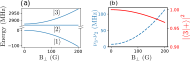
\includegraphics[width=\textwidth]{Figures/transis_transverse_field}
\caption{Simulation of the eigenstates of the NV Hamiltonian for $d_\perp E_perp=4\ \rm MHz$ and a purely transverse magnetic field $B_\perp$. (a) Eigenvalues for the spin Hamiltonian as a function of $B_\perp$. The three states are labeled $\ket{1}$, $\ket{2}$ and $\ket{3}$ (b) Splitting between the $\ket{2}$ and $\ket{3}$ states (blue curve) and closeness factor $\abs{\bra{3}\ket{+}}^2$ between the $\ket{3}$ and $\ket{+}$ (red curve)}
\label{eigenstates transverse field}
\end{figure}

Fig. \ref{eigenstates transverse field} shows a simulation of the eigenstates and eigenenergies for a NV Hamiltonian subject to transverse electric field and magnetic field. For convenience we chose to take $E_\perp = E_x$ and $B_\perp = B_x$, taking other geometric configuration only alters slightly the results. We labeled the eigenstates of the Hamiltonian $\ket{1}$, $\ket{2}$ and $\ket{3}$ in ascending order of energy.

Fig. \ref{eigenstates transverse field}-b) shows both the splitting $\Delta \nu$ between the $\ket{2}$ and $\ket{3}$ states, and how close the $\ket{3}$ state is to the $\ket{+}=\frac{\ket{+1}+\ket{-1}}{\sqrt{2}}$ state via the factor $\abs{\bra{3}\ket{+}}^2$. We look at the $\ket{3}$ state since $\ket{2}=\ket{-}=\frac{\ket{+1}-\ket{-1}}{\sqrt{2}}$ in this case.

These two metrics, $\Delta \nu$ and $\abs{\bra{3}\ket{+}}^2$ are what we are interested in: we want to increase $\Delta \nu$ to the point where the double flips are completely quenched, but we want $\abs{\bra{3}\ket{+}}^2$ to remain close to 1 since we wanted to observe the modification caused by the eigenbasis $\{\ket{0},\ket{\pm}\}$. This way we can isolate the $T_1^{\rm dd}$ contribution coming from the change of eigenstates to the one coming from the double flips. Based on the plots in Fig.\ref{eigenstates transverse field}-b), the region with $B_\perp \in$ [100,200] G seems to satisfy both these criteria.

\subsection{Experimental data}

\begin{figure}[h!]
\centering
\includegraphics[width=.8\textwidth]{Figures/scan_T1_perp}
\caption{Experimental data for the depolarization under purely transverse magnetic field on sample ADM-150-2. a) ODMR spectrum for $|\mathbf{B}|=20\ \rm G$. The transitions of the class orthogonal to the magnetic field are labeled $\nu_+$ and $\nu_-$. b) Dependency of $\nu_+$ and $\nu_-$ with the magnetic field, as measured through ODMR. c) Measurement of $T_1^{\rm dd}$ as a function of the transverse magnetic field. The corresponding energy splittings $\Delta \nu=\nu_+-\nu_-$ are written on top. We divided the plot between the A region where $1/T_1^{\rm dd}$ decreases, and the B region where it reaches a plateau with a value $1/T_1^{\rm dd}=185 \pm 5\ \rm s^{-1}$ indicated by a red line. We also indicate in green the value found for a purely longitudinal magnetic field $1/T_1^{\rm dd}=126 \pm 10\ \rm s^{-1}$}
\label{champ tranverse exp}
\end{figure}

We perform here a $T_1^{\rm dd}$ measurement similar to the one presented in Fig. [REF], on the same sample and with the same fitting parameters, but this time probing a class orthogonal to the magnetic field.

Fig. \ref{champ tranverse exp}-a) and b) show the evolution of the transition frequencies $\nu_+=\frac{E_{\ket{3}}-E_{\ket{1}}}{h}$ and $\nu_-=\frac{E_{\ket{2}}-E_{\ket{1}}}{h}$ where $\ket{1}$, $\ket{2}$ and $\ket{3}$ are the states described in Fig. \ref{eigenstates transverse field}. The magnetic field was scanned between 20 and 130 G by increment of $\sim 0.5\ \rm G$.

Fig. \ref{champ tranverse exp}-c) shows the evolution of $1/T_1^{\rm dd}$ with the magnetic field. We have denoted two region: in region A, $1/T_1^{\rm dd}$ decreases with the magnetic field, from a value of $350\ \rm s^{-1}$ to a value of $185\ \rm s^{-1}$. In region B, the $1/T_1^{\rm dd}$ value is stable and does not decrease further when $B_\perp$, or $\Delta \nu$ are increased.

We attribute the decrease in region A to the double flips: as the magnetic field and $\Delta \nu$ are increased, the double flips become less and less resonant to the point where they become completely quenched for $B_\perp \approx 90\ \rm G$ or $\Delta \nu \approx 30\ \rm MHz$. This value is coherent with the previously measured fluctuator linewidth. We can then estimate the part of the double flips in the low field (20 G here) depolarization rate and find that they amount for $\sim 50\%$ in this case.

Another possibility to explain this drop could be that the class orthogonal to $\mathbf{B}$ still exerts flip-flops with the other classes at low magnetic field, as we can see that they are not very far detuned in Fig. \ref{champ tranverse exp}-a), but we have to consider that the detuning between the two states $\nu_+-\nu_-= 9\ \rm MHz$ is significantly lower, even at $B_\perp=20\ \rm G$, than the detuning with the closest class $\nu_\pm-\nu_{\rm other}= 22\ \rm MHz$; and also that there seem to be a small plateau for $1/T_1^{\rm dd}$ at the beginning of region A, which is consistent with the double flip hypothesis since  $\nu_+-\nu_-$ is almost flat in this region while $\nu_\pm-\nu_{\rm other}$ increases linearly with the magnetic field.

We now turn to region B. Even tough the double flips are completely quenched, the effects of the eigenbasis modification and the $T_2^*$ reduction are still present, because we can see on Fig. \ref{eigenstates transverse field}-b) that the eigenstates of the spin Hamiltonian are still very close to $\{ \ket{0}, \ket{\pm} \}$ for these magnetic field values.

Indeed, when we compare the plateau value $1/T_1^{\rm dd}=185 \pm 5\ \rm s^{-1}$ to the value $1/T_1^{\rm dd}=126 \pm 10\ \rm s^{-1}$ found with a longitudinal magnetic field, we notice an increase by $\sim 50\%$ of the depolarization rate. This is in agreement with the theory which predicts an increase of the decay rate in the $\ket{\pm}$ basis compared to the $\ket{\pm 1}$ basis, although the theoretical increase, when considering only the change of eigenbasis, is a factor of 4 (see appendix [REF]). We again find the the theory significantly overestimates the measured decay rates, although this discrepancy could still come from the fitting procedure.

We unfortunately cannot experimentally discriminate the depolarization coming from the eigenbasis change or the $T_2^*$ while using the same sample, since both of this properties are tied to the Hamiltonian eigenstates. We do know however that the double flips seem to play a more important role in the low field depolarization, even in a regime where the eigenbasis change should play an important role (we expect $\Gamma_1^{\ket{\pm}}=4 \Gamma_1^{\ket{\pm}}$ for a single class, but only $\Gamma_1^{\ket{\pm}}\approx 1.2 \Gamma_1^{\ket{\pm}}$ when the 4 classes are resonant).


\section{Low field magnetometry}

Ne pas oublier (ou alors en perspective, c'est bien aussi) : les deux adamas du 20210927 avec le petit et le gros DQ

\section{Conclusion and perspectives}
- Improvement to the sensitivity : Scale up, material optimization (15N !)

- Understand the impact of the various factors on the flip-flop CR and DQ CR: T2*, strain, local electric noise ...

- Application for uneven surfaces, polycrystalline heteroepithaxy, low/no microwave environment (dimaond anvil cells, bio sensing)

\printbibliography
\end{document}
